%%%%%%%%%%%%%%%%%%%%%%%%%%%%%%%%%%%%%%%%%
% Beamer Presentation
% LaTeX Template
% Version 1.0 (10/11/12)
%
% This template has been downloaded from:
% http://www.LaTeXTemplates.com
%
% License:
% CC BY-NC-SA 3.0 (http://creativecommons.org/licenses/by-nc-sa/3.0/)
%
%%%%%%%%%%%%%%%%%%%%%%%%%%%%%%%%%%%%%%%%%

%----------------------------------------------------------------------------------------
%	PACKAGES AND THEMES
%----------------------------------------------------------------------------------------

\documentclass{beamer}

\mode<presentation> {

%\usetheme{default}
%\usetheme{AnnArbor}
%\usetheme{Antibes}
%\usetheme{Bergen}
%\usetheme{Berkeley}
%\usetheme{Berlin}
%\usetheme{Boadilla}
\usetheme{CambridgeUS}
%\usetheme{Copenhagen}
%\usetheme{Darmstadt}
%\usetheme{Dresden}
%\usetheme{Frankfurt}
%\usetheme{Goettingen}
%\usetheme{Hannover}
%\usetheme{Ilmenau}
%\usetheme{JuanLesPins}
%\usetheme{Luebeck}
%\usetheme{Madrid}
%\usetheme{Malmoe}
%\usetheme{Marburg}
%\usetheme{Montpellier}
%\usetheme{PaloAlto}
%\usetheme{Pittsburgh}
%\usetheme{Rochester}
%\usetheme{Singapore}
%\usetheme{Szeged}
%\usetheme{Warsaw}

% As well as themes, the Beamer class has a number of color themes
% for any slide theme. Uncomment each of these in turn to see how it
% changes the colors of your current slide theme.

%\usecolortheme{albatross}
%\usecolortheme{beaver}
%\usecolortheme{beetle}
%\usecolortheme{crane}
%\usecolortheme{dolphin}
%\usecolortheme{dove}
%\usecolortheme{fly}
%\usecolortheme{lily}
%\usecolortheme{orchid}
\usecolortheme{rose}
%\usecolortheme{seagull}
%\usecolortheme{seahorse}
%\usecolortheme{whale}
%\usecolortheme{wolverine}

%custom footline
\setbeamertemplate{footline}
{
  \leavevmode%
  \hbox{%
  \begin{beamercolorbox}[wd=.333333\paperwidth,ht=2.25ex,dp=1ex,center]{author in head/foot}%
    \usebeamerfont{author in head/foot}\insertshortauthor
  \end{beamercolorbox}%
  \begin{beamercolorbox}[wd=.333333\paperwidth,ht=2.25ex,dp=1ex,center]{title in head/foot}%
    \usebeamerfont{title in head/foot}\insertshortinstitute
  \end{beamercolorbox}%
  \begin{beamercolorbox}[wd=.333333\paperwidth,ht=2.25ex,dp=1ex,right]{date in head/foot}%
    \usebeamerfont{date in head/foot}\insertshortdate{}\hspace*{2em}
    \insertframenumber{} / \inserttotalframenumber\hspace*{2ex} 
  \end{beamercolorbox}}%
  \vskip0pt%
}

% change bullet point style
\setbeamertemplate{items}[circle]

% set left and right margins
\setbeamersize{text margin left=12mm,text margin right=12mm}

% remove nav
\setbeamertemplate{navigation symbols}{}
}

% use unicode
\usepackage[utf8]{inputenc}

% use tikz
\usepackage{tikz}

% korean characters
\usepackage{CJKutf8}

% set math font to serif
\usefonttheme[onlymath]{serif}

\usepackage{bm}
\usepackage{amsmath}
\usepackage{amssymb}
\usepackage{graphicx} % Allows including images
\usepackage{booktabs} % Allows the use of \toprule, \midrule and \bottomrule in tables

%----------------------------------------------------------------------------------------
%	TITLE PAGE
%----------------------------------------------------------------------------------------

\title{Bridging the Gap between Training and Inference for Neural Machine Translation}
\author[Bj\"orn Bebensee]{
    Wen Zhang, Yang Feng, Fandong Meng, Di You, Qun Liu\\
    \bigskip
    Bj\"orn Bebensee\\
    \medskip
    {\tt bebensee@bi.snu.ac.kr} 
}
\institute[Biointelligence Laboratory]{
    %$\vcenter{\hbox{
\includegraphics[width=0.1\textwidth]{bi.png}}}$
    \normalsize Biointelligence Laboratory
}
\date{November 14, 2019}

\begin{document}

\begin{frame}
    \titlepage
\end{frame}

\begin{frame}
    \frametitle{Overview}
    \tableofcontents
\end{frame}

%----------------------------------------------------------------------------------------
%	PRESENTATION SLIDES
%----------------------------------------------------------------------------------------

%------------------------------------------------
%------------------------------------------------

\section{Introduction}

\subsection{Background}

%------------------------------------------------

\begin{frame}
    \frametitle{A brief introduction to NMT}

\end{frame}

%------------------------------------------------

\begin{frame}
    \frametitle{A brief introduction to NMT}

\end{frame}

%------------------------------------------------

\begin{frame}
    \frametitle{A brief introduction to NMT}

\end{frame}

%------------------------------------------------

\begin{frame}
    \frametitle{A brief introduction to NMT}
    \textbf{Notation:}\\
    \bigskip
    Source sequence $x = \{ x_1, \ldots, x_{|x|} \}$\\
    \medskip
    Word embeddings $e_{x_i}$ for each $x_i \in x$\\
    \medskip
    Observed translation $y^* = \{ y_1^*, \ldots, y^*_{|y^*|} \}$
\end{frame}

%------------------------------------------------

\begin{frame}
    \frametitle{A brief introduction to NMT}
    \textbf{Encoder:} bidirectional Gated Recurrent Unit (GRU), obtain hidden states $h_i = [ \ \overset{\rightarrow}{h_i}; \overset{\leftarrow}{h_i} \ ]$ where
    \begin{align}
        \overset{\rightarrow}{h_i} &= \bm{\mathrm{GRU}}(e_{x_i}, \overset{\rightarrow}{h_{i-1}})\\
        \overset{\leftarrow}{h_i} &= \bm{\mathrm{GRU}}(e_{x_i}, \overset{\leftarrow}{h_{i+1}})
    \end{align}
\end{frame}

%------------------------------------------------

\begin{frame}
    \frametitle{A brief introduction to NMT}
    \textbf{Attention:} attention over source/target words:
    \begin{gather} 
        r_{ij}=\bm{\mathrm{v}}_a^T \tanh\left(\bm{\mathrm{W}}_as_{j-1} + \bm{\mathrm{U}}_ah_i\right) \label{eq:att_query} \\
        \alpha_{ij} = \frac{\exp \left( r_{ij} \right)}{\sum_{i'=1}^{|\bm{\mathrm{x}}|} \exp \left( r_{i'j} \right)} \label{eq:att_alpha}
    \end{gather}
    Yields ``source context vector" $c_j$ at the $j$-th time step as a weighted sum of all source annotations:
    \begin{gather}
        c_j = \sum\nolimits_{i=1}^{|\bm{\mathrm{x}}|}\alpha_{ij}h_i
    \end{gather}
\end{frame}

%------------------------------------------------

\begin{frame}
    \frametitle{A brief introduction to NMT}
    \textbf{Decoder:} another GRU, given the source context vector $c_j$ ``unrolls" the target hidden state $s_j$ at time step $j$:
    \begin{equation}
        s_j = \bm{\mathrm{GRU}}(e_{y_{j-1}^{*}}, s_{j-1}, c_j)
    \end{equation}
    Gives probability distribution $P_j$ over all words in the target vocabulary as follows:
    \begin{gather}
        t_j = g\left(e_{y_{j-1}^{*}}, c_j, s_j\right)  \label{eq:t} \\
        o_j = \bm{\mathrm{W}}_o t_j \label{eq:o} \\
        P_{j} = \mathrm{softmax}\left(o_j\right)  \label{eq:softmax}
    \end{gather}
\end{frame}

%------------------------------------------------

\subsection{Motivation}

\begin{frame}
    \frametitle{Motivation}
    NMT models are trained to predict the next word, given the previous context words.\\
    \bigskip
    Learn a distribution!
\end{frame}

%------------------------------------------------

\begin{frame}
    \frametitle{Motivation}
    \textbf{However:}\\
    \bigskip
    \textbf{At training time:} model uses ground truth words as context to predict the next word (context from data distribution)\\
    \bigskip
    \textbf{At inference time:} model uses own previous predictions as context (context from model distribution)\\
    \bigskip
    This gap is called \emph{exposure bias}.
\end{frame}

%------------------------------------------------

\begin{frame}
    \frametitle{Motivation}
    Training typically uses cross-entropy loss, optimizes target sequence to fit ground truth sequence as closely as possible.\\
    \bigskip
    \textbf{Problem:} one sentence can have multiple possible translations.\\
    \medskip
    \begin{tabular}{ll}
        \centering
        {\em reference}: & We should comply with the rule. \\
        {\em cand1}: & We should abide with the rule. \\
        {\em cand2}: & We should abide by the law. \\
        {\em cand3}: & We should abide by the rule. \\
    \end{tabular}\\
    \bigskip
    Loss forces prediction back to ground truth (\emph{overcorrection}).
\end{frame}

%------------------------------------------------

\section{Contributions}

\subsection{Overview}

\begin{frame}
    \frametitle{Contributions}
    Introduce a method that ``bridges the gap" between training and inference.\\
    \bigskip
    Improves the model's ability to recover from overcorrection and overall performance.
\end{frame}

%------------------------------------------------

\subsection{Proposed method}

\begin{frame}
    \frametitle{Proposed method}
    \textbf{Simple idea:} Instead of just ground truth, feed the model either previous predicted words or ground truth with a certain probability.\\
    \bigskip
    Brings training conditions closer to inference time.
\end{frame}

%------------------------------------------------

\begin{frame}
    \frametitle{Proposed method}
    \begin{figure}
        \centering
        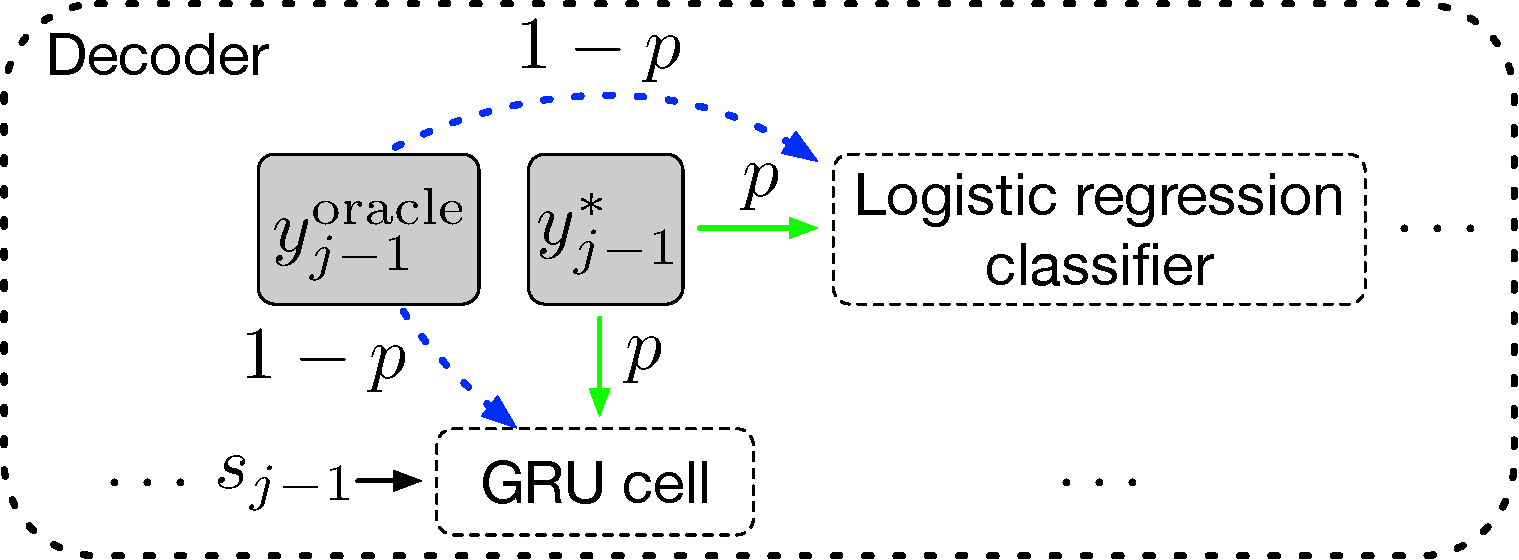
\includegraphics[width=\textwidth]{fig/decoder-p.pdf}
        \caption{Sample between ground truth word and oracle word}
    \end{figure} 
\end{frame}

%------------------------------------------------

\begin{frame}
    \frametitle{Proposed method}
    To predict $j$-th target word $y_j$:\\
    \bigskip
    \only<1>{
        Recall:
        \begin{gather*}
            s_j = \bm{\mathrm{GRU}}(e_{y_{j-1}^{*}}, s_{j-1}, c_j)\\
            P_j = \mathrm{softmax}\left(
                \bm{\mathrm{W}}_o \
                g\left(e_{y_{j-1}^{*}}, c_j, s_j\right)
            \right)
        \end{gather*}
        where $s_j$ next hidden state and $P_j$ probability distribution over target vocabulary 
    }
    \only<2->{
        \begin{itemize}
        \item[1.] Select an oracle word $y_{j-1}^\mathrm{oracle}$ at the \{$j$$-$$1$\}-th step.
        \item[2.] Sample from the ground truth word $y_{j-1}^*$ with a probability of $p$ or from the oracle word $y_{j-1}^\mathrm{oracle}$ with a probability of $1$$-$$p$.
        \item[3.] Use the sampled word as context $e_{y_{j-1}^{*}}$.
        \end{itemize}
    }
\end{frame}

%------------------------------------------------

\subsection{Oracle word selection}

\begin{frame}
    \frametitle{Oracle word selection}
    Two strategies to select the oracle words:\\
    \bigskip
    \begin{itemize}
        \item[1.] word-level oracle (greedy search)
        \item[2.] sentence-level oracle (select an oracle sequence)
    \end{itemize}
\end{frame}

%------------------------------------------------

\begin{frame}
    \frametitle{Word-level Oracle}
    Easiest way to pick an oracle word: pick the word with highest probability from the distribution $P_{j-1}$
    \begin{figure}
        \centering
        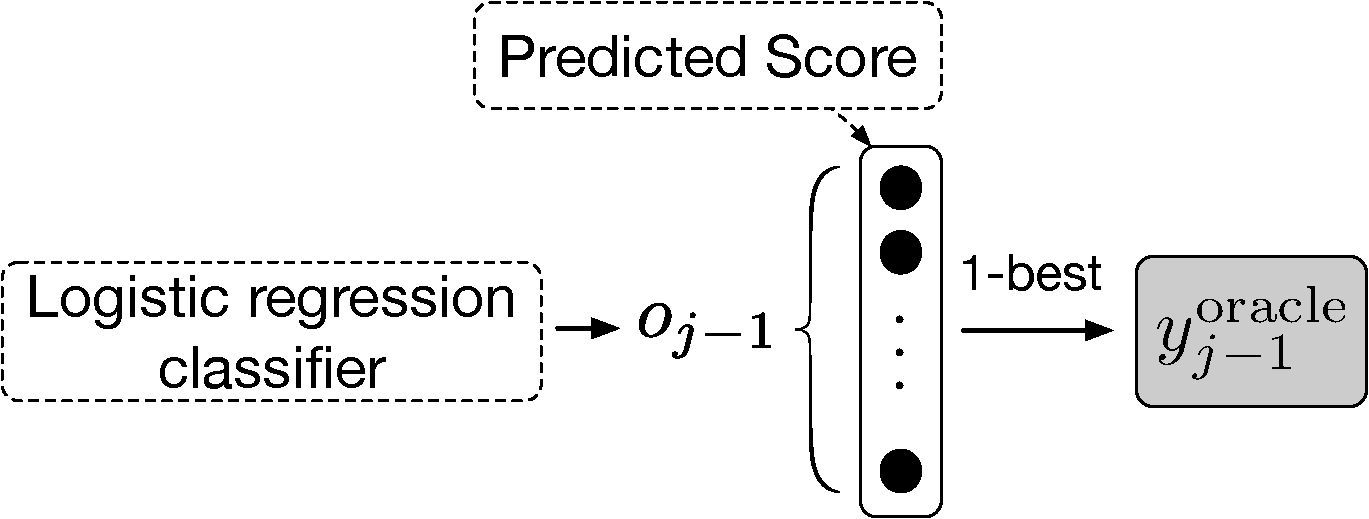
\includegraphics[width=\textwidth]{fig/wonoise.pdf}
        \caption{Word-level oracle without noise}
    \end{figure}
\end{frame}

%------------------------------------------------

\begin{frame}
    \frametitle{Word-level Oracle}
    Better: Add noise to the the scores for a better sample
    \begin{figure}
        \centering
        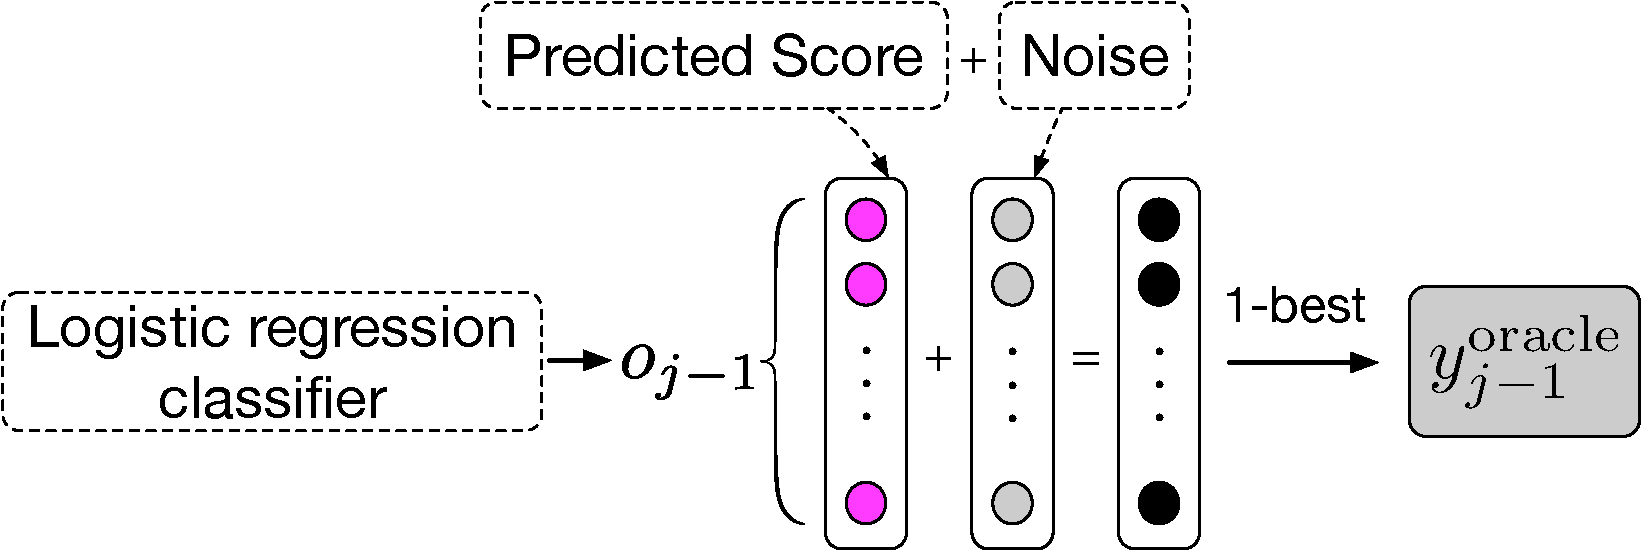
\includegraphics[width=\textwidth]{fig/oracle_noise.pdf}
        \caption{Word-level oracle with Gumbel noise}
    \end{figure}
\end{frame}

%------------------------------------------------

\begin{frame}
    \frametitle{Word-level Oracle}
    \begin{exampleblock}{\emph{Gumbel-Max} technique:}
        Simple, efficient way to sample from categorical distribution
    \end{exampleblock}
    \bigskip
    Given Gumbel noise $\eta$ and a temperature $\tau$, obtain
    \begin{align}
        \tilde{o}_{j-1} &= \left(o_{j-1} + \eta\right)/\tau\\
        \tilde{P}_{j-1} &= \mathrm{softmax}(\tilde{o}_{j-1})
    \end{align}
    and select the 1-best word from $\tilde{P}_{j-1}$.\\
    \bigskip
    Optimal temperature: $\tau = 0.5$ (found in experiments)
\end{frame}

%------------------------------------------------

\begin{frame}
    \frametitle{Sentence-level Oracle}
    Enlarge the search space: perform beam search, apply Gumbel noise at every word generation and get $k$-best candidate translations\\
    \bigskip
    Rank candidates according to some sentence-level metric (here: BLEU), best sentence is used as \emph{oracle sentence}
\end{frame}

%------------------------------------------------

\begin{frame}
    \frametitle{Force Decoding}
    \begin{alertblock}{Problem}
        What if oracle sentence and ground truth do not have the same length?
    \end{alertblock}
    \bigskip
    Use \textbf{force decoding} to force oracle sentence length to be $|y^*|$ (length of ground truth). Modify beam search as follows:\\
    \bigskip
    If $j \leq |y^*|$ and top first word is \texttt{<EOS>}: select second word in $\tilde{P}_j$ for this candidate sentence\\
    \bigskip
    If \texttt{<EOS>} not top first word in $\tilde{P}_{|y^*|+1}$: select \texttt{<EOS>} as $\{|y^*|+1 \}$-th word for this candidate sentence
\end{frame}

%------------------------------------------------

\begin{frame}
    \frametitle{Sampling with decay}
    Convergence of the model depends on the choice of sampling probability $p$.\\
    \bigskip
    $p$ too low: Sample from the ground-truth too often\\
    \smallskip
    $p$ too high: Slow or no convergence
\end{frame}

%------------------------------------------------

\begin{frame}
    \frametitle{Sampling with decay}
    Let $p$ decay as training progresses so we progressively sample more often from the model distribution and select oracle words.\\
    \bigskip
    Start with $p=1$. Define it dependent on training epoch $e$:\\
    \begin{gather}
        p = \frac{\mu}{\mu + \mathrm{exp}(e/\mu)}
    \end{gather}
    with hyperparameter $\mu$.
\end{frame}

%------------------------------------------------

\section{Evaluation}

\subsection{Comparison}

\begin{frame}
    \frametitle{Evaluation}
    \begin{figure}
        \centering
        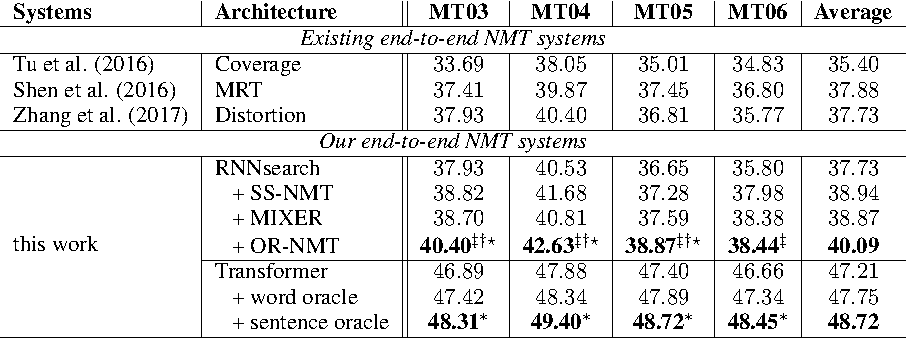
\includegraphics[width=\textwidth]{fig/bleu_table}
        \caption{
            Case-insensitive BLEU scores (\%) on Zh$\rightarrow$En translation task. %``$\ddag$", ``$\dag$", ``$\star$" and ``$\ast$" indicate statistically significant difference (p\textless0.01) from RNNsearch, SS-NMT, MIXER and Transformer, respectively.
        }
    \end{figure}
\end{frame}

%------------------------------------------------

\subsection{Factor analysis}

\begin{frame}
    \frametitle{Factor analysis}
    \begin{figure}
        \centering
        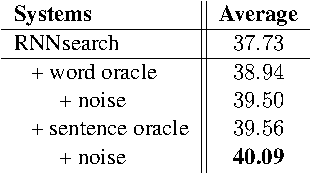
\includegraphics[width=0.5\textwidth]{fig/factor_analysis_table.pdf}
        \caption{Factor analysis on Zh$\rightarrow$En translation, the results are average BLEU scores on MT03$\sim$06 datasets.}
    \end{figure} 
\end{frame}

%------------------------------------------------

\subsection{Convergence}

\begin{frame}
    \frametitle{Convergence}
    \begin{columns}[T]
        \begin{column}{0.48\textwidth}
            \begin{figure}
                \centering
                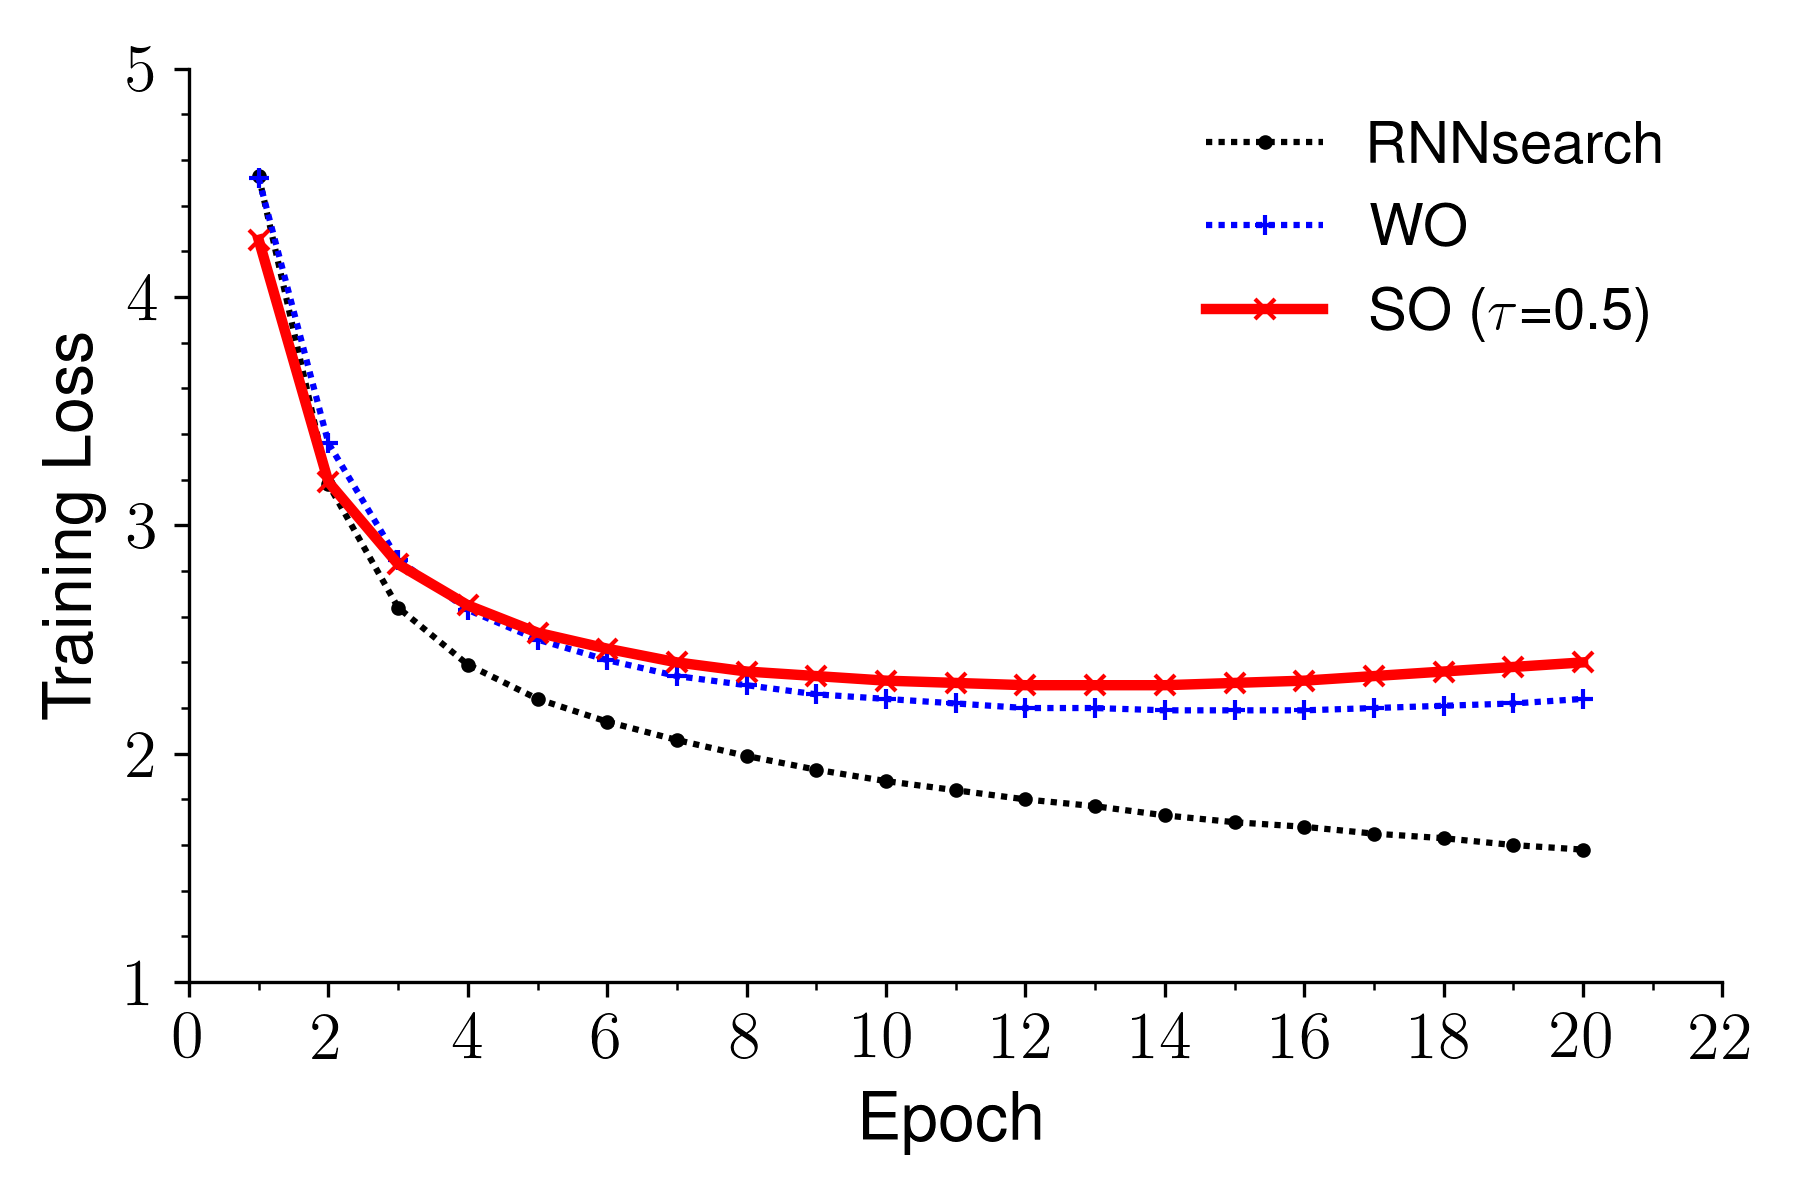
\includegraphics[width=\textwidth]{fig/training_curve_loss.png}
            \end{figure}
        \end{column}
        \begin{column}{0.48\textwidth}
            \begin{figure}
                \centering
                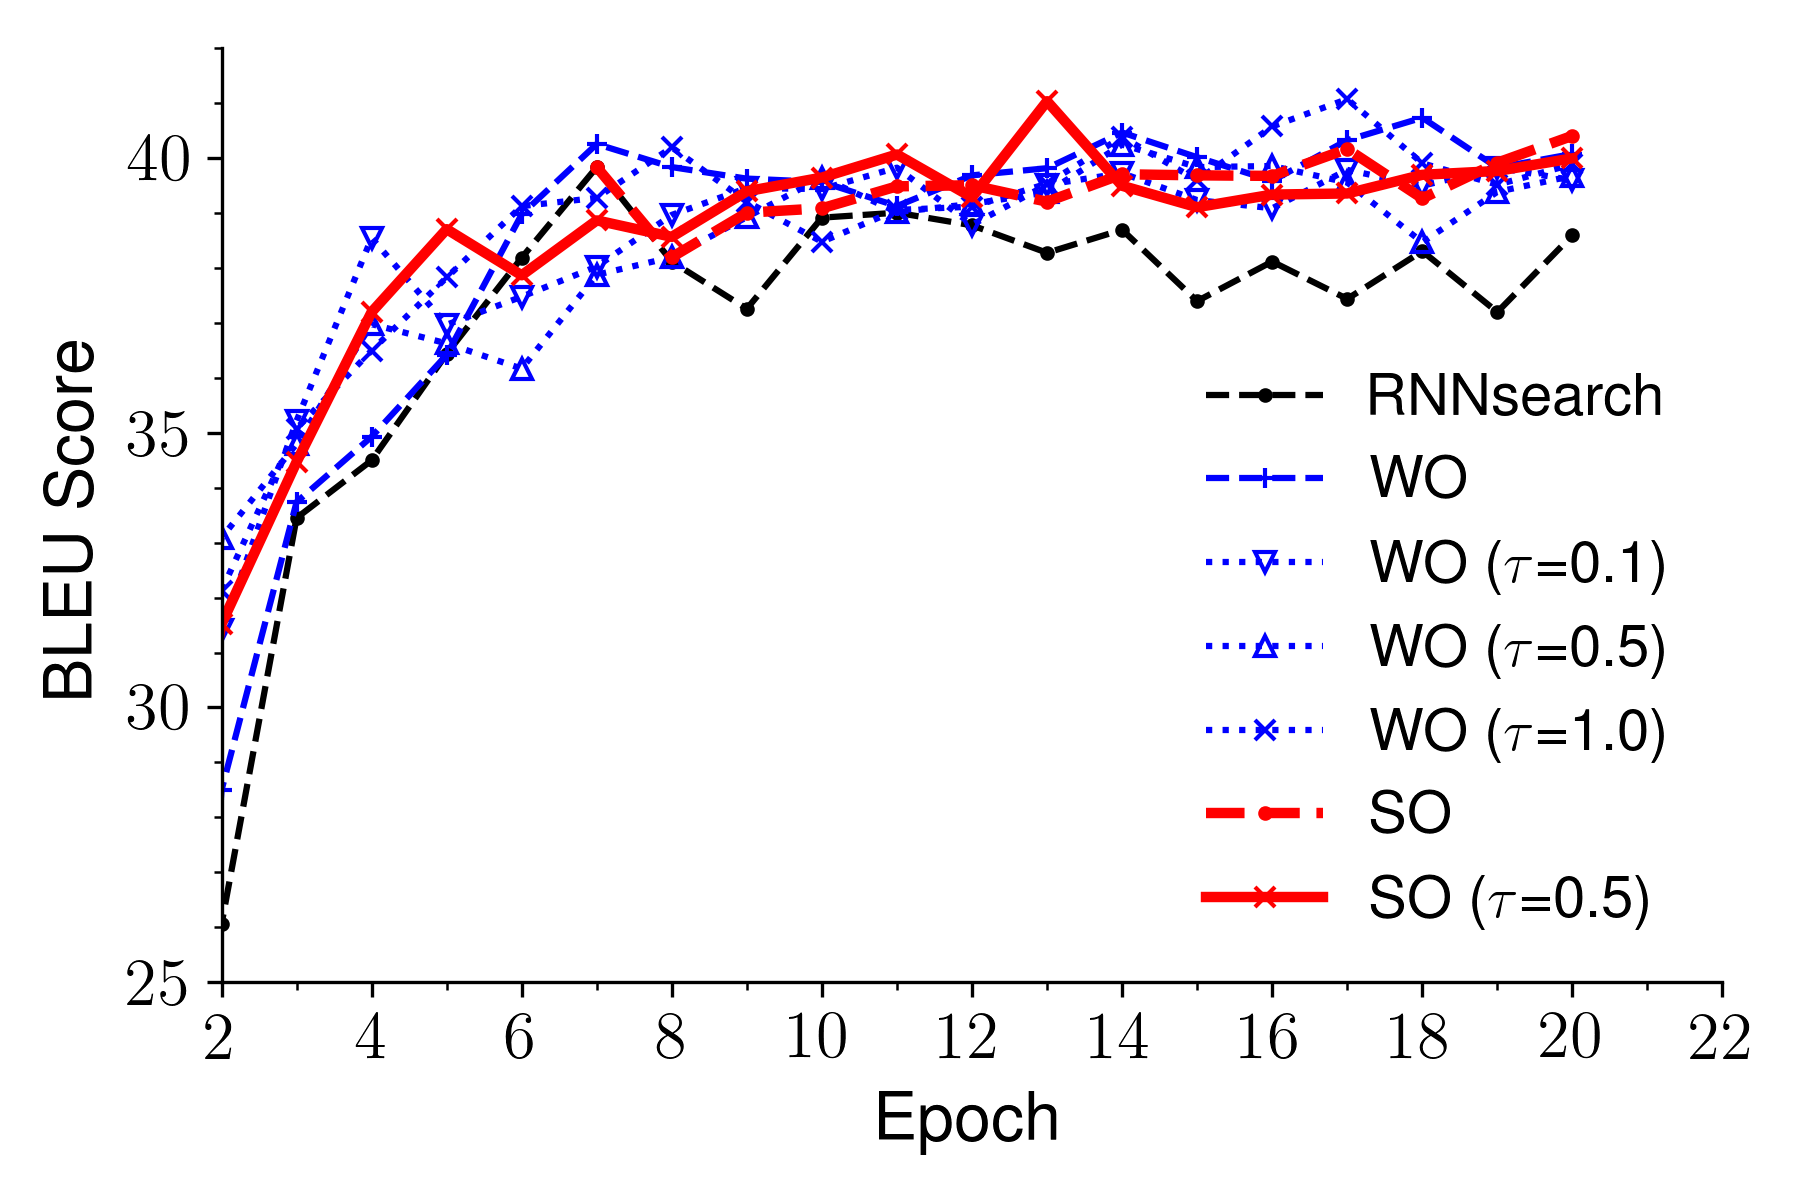
\includegraphics[width=\textwidth]{fig/dev_curve_bleu.png}
            \end{figure}
        \end{column}
    \end{columns}
    Slower convergence but loss does not keep decreasing (intuition: WO and SO models help avoid overfitting)
\end{frame}

%-----------------------------------------------

\subsection{Sentence length}

\begin{frame}
    \frametitle{Sentence length analysis}
    \begin{figure}
        \centering
        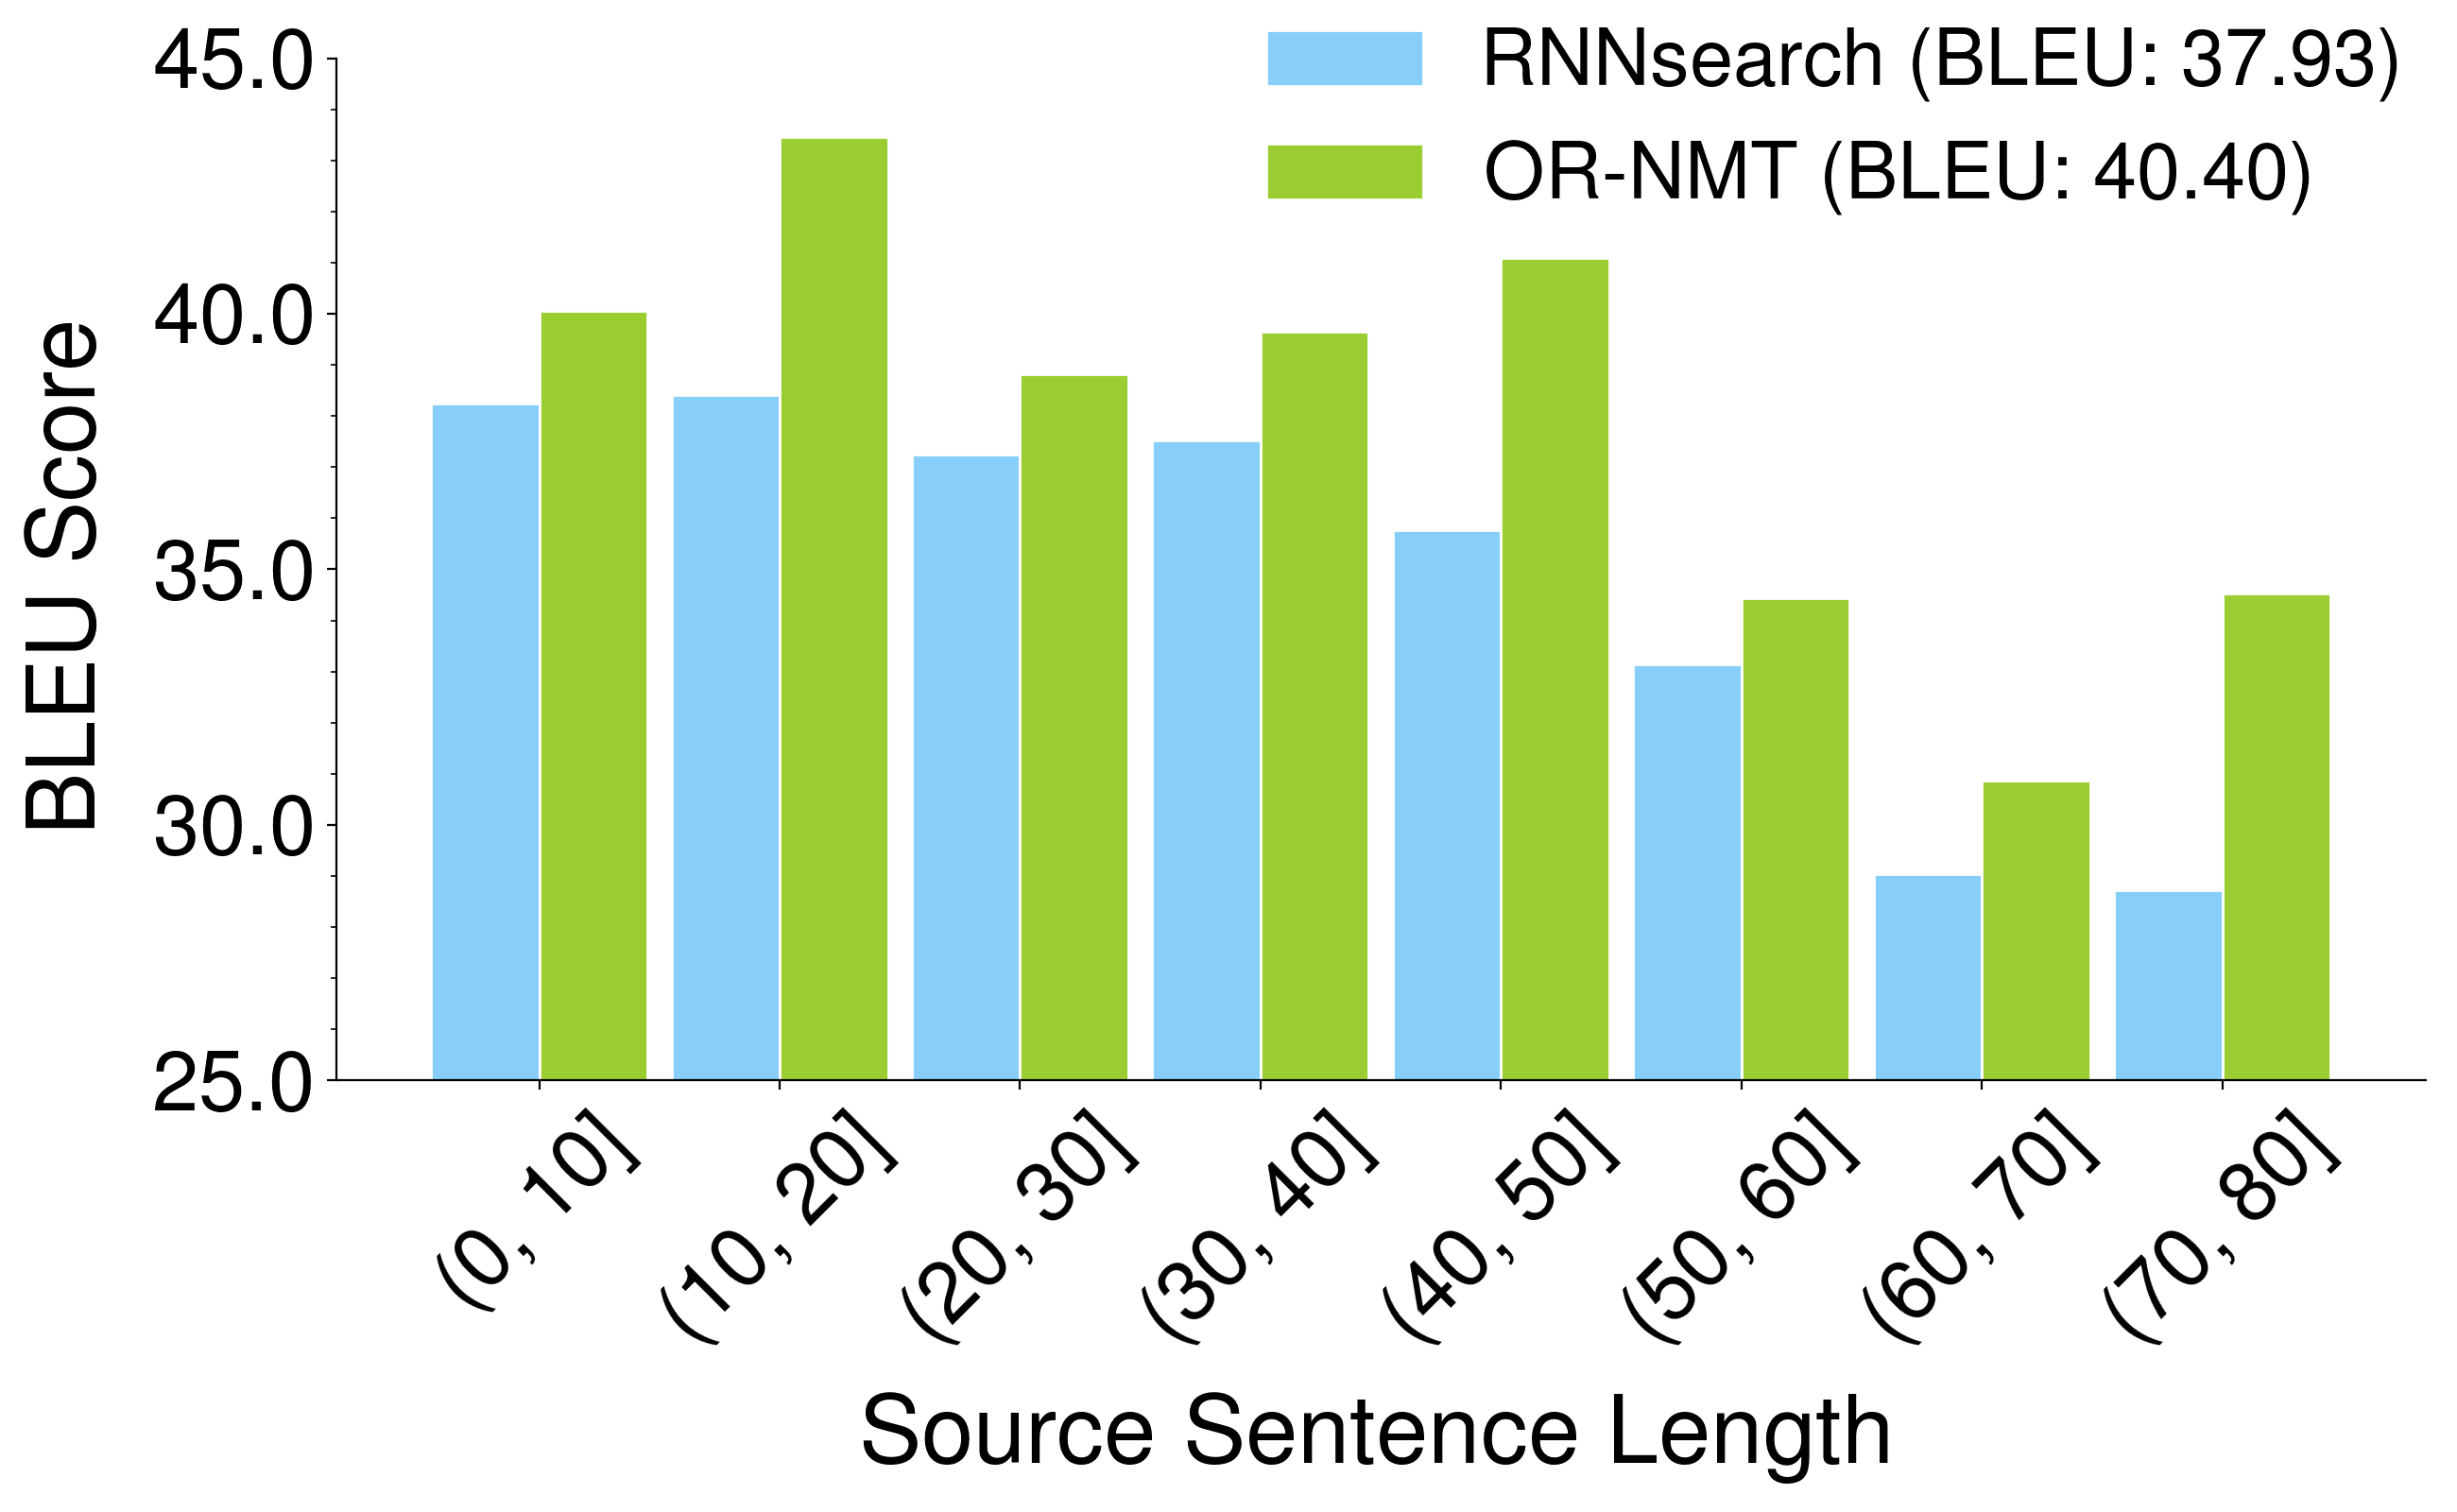
\includegraphics[width=0.7\textwidth]{fig/length.png}
        %\caption{MT03 test set, Zh$\rightarrow$ En}
    \end{figure}
    Cross-entropy loss requires predicted sequence to be same as ground truth, difficult for long sentences! Oracle helps recover from overcorrection
\end{frame}

%-----------------------------------------------

\section{Conclusion}

\begin{frame}
    \frametitle{Conclusion}
    To conclude: Zhang et al. proposed a new training technique that helps to recover from overcorrection.\\
    \bigskip
    Outperforms previous methods as well as the transformer baseline.\\
    \bigskip
    Technique can be used with a variety of models.
\end{frame}

%-----------------------------------------------

\begin{frame}
    \Large{\centerline{Thank you for your attention.}}
\end{frame}

%----------------------------------------------------------------------------------------

\end{document}